\chapter{Materiales y métodos}\label{C:Materiales}
\graphicspath{{./figs/02_Mat/}}
\section{Experimentos de difracción de rayos X}\label{S:MatXRD}
Buena parte del trabajo de esta tesis se centró alrededor de los experimentos de difracción de rayos X.
En particular, la mediciones se hicieron empleando la geometría de transmisión, también llamada de Debye-Scherrer, utilizando radiación sincrotrón.
La facilidad empleada fue PETRA III, cuya fotografía puede verse en la Fig. \label{fig:desy}, y está ubicada en el complejo DESY, en la ciudad de Hamburgo, Alemania\cite{desy}.

\begin{figure}[!htb]
  \centering
  \includegraphics[width=\textwidth]{desy}
  \caption{Fotografías del exterior e interior de la facilidad PETRA III, en DESY. Imágenes obtenidas de \cite{desy}.}
  \label{fig:desy}
\end{figure}

En los experimentos de transmisión realizados, un haz de rayos X con $\lambda \ \approx \ 0.0142$\,nm incide sobre una dada muestra, como se puede apreciar en la imagen de la Fig. \ref{fig:transmision}. 
Como resultado de la interacción elástica entre el haz incidente y el material, diferentes haces con la misma energía que el incidente, son dispersados por diferentes familias de planos en ángulos que están dados por la Ley de Bragg \ref{eq:Bragg}.
Para una dada familia de planos $\{hkl\}$ todos los haces difractados están comprendidos en un cono, que al interceptar el detector forman un círculo, denominado anillo de Debye, y la intensidad del haz difractado a lo largo de largo del anillo de Debye está determinada por la cantidad de planos cristalinos en condición de difracción para esa dada orientación de la muestra.

En la configuración que se muestra en la Fig. \ref{fig:transmision} la muestra se colocó en un portamuestra que permitía la alineación con el haz y el detector, y daba a la muestra la libertad de girar alrededor de un eje vertical que pasaba por su centro.
La muestra rotaba gracias a un motor paso a paso y que permitía rotar con una precisión de 5\,$^{\circ}$.
Para obtener una caracterización completa de la textura de la muestra, fue necesario rotar la misma un rango de 180\,$^{\circ}$, lo que sumado a la resolución en la rotación significa que por cada muestra se obtuvieron 37 anillos de Debye.

\begin{figure}[!htb]
  \centering
  \includegraphics[width=\textwidth]{process}
  \caption{Esquema básico del proceso de medición y análisis de datos. Las mediciones se realizaron empleando una geometría de transmisión, para diferentes rotaciones $\omega$ de la muestra. Por cada posición de la muestra se registraron una serie de anillos de Debye, a partir de los cuales se extrajeron porciones radiales con los que se construyeron los difractogramas que luego fueron procesados siguiendo diferentes modelos microestructurales. A partir de estos resultados, y realizando la conversión adecuada de las coordenadas de laboratorio a las coordenadas del sistema de referencia del cristal, se construyeron figuras de polos y figuras de polos generalizadas.}
  \label{fig:transmision}
\end{figure}

El haz que incidente tiene un tamaño de 100\,$\mu$m x 100\,$\mu$m, lo que permite obener una gran resolución sobre la microestructura del material.
Las muestras empleadas tenían forma de varillas con su eje colocado verticalmente, es decir, paralelas al eje de giro.
El ancho de las varillas era de entre 2\,mm y 5\,mm, y se tuvo especial cuidado durante la alineación de que el haz esté completamente adentro de la muestra en todo el rango de rotación de la muestra.
Se utilizó un detector de estado sólido Mar345 de forma cuadrada, con una grilla de 3450\,pixels x 3450\,pixels, de 100\,$\mu$m x 100\,$\mu$m cada uno.
El detector se colocó 1081\,mm detrás de la muestra, y los tiempos de detección se modificaron de acuerdo a la intensidad de salida del haz y la absorción de la muestra, de modo de que las intensidades máximas siempre estén cerca del número máximo de cuentas medibles por el detector.

De cada medición se extrajeron 37 imágenes, cada una de las cuales contaba con conjuntos de 5 a 7 anillos de Debye, dependiendo de la muestra.
De cada imagen se extrajeron porciones radiales de ancho angular de 5\,$^{\circ}$ a partir de las cuales se construyeron 72 difractogramas.
El conjunto de 72 x 37 = 2664 difractogramas fue analizado utilizando diferentes modelos microestructurales, pero hubo dos modelos sobre los que se hizo especial foco: el CMWP (Sec. \ref{SS:CMWP}) y el de Langford (Sec. \ref{SS:02Langford}), y de cada modelo empleado se extrajo diferente información sobre la microestructura.

Cada pico de cada difractograma quedaba identificado por su ánglulo de Bragg $\theta_B$, su coordenada angular $\gamma$ en el anillo de Debye y la rotación de la muestra $\omega$ cuando se realizó la medición, por lo que la información microestructural era susceptible de ser graficada empleando figuras de polos, del misma manera que se grafican las figuras de polos.
Para construir figuras de polos a partir de las mediciones realizadas es preciso transformar las coordenadas de los picos en el sistema de laboratorio $(\omega, \gamma, \theta_B)$ al sistema de referencia del cristal $(\alpha, \beta)$, para lo cual se empleó la matriz de rotación ya calculada por Bunge y Klein\cite{Bunge1996}.
La misma expresión fue empleada para generar las figuras de polos generalizadas.

\subsection{Contribuciones instrumentales al ancho de pico}\label{SS:inst}
Para poder realizar un análisis microestructural preciso a partir de mediciones de ancho de pico, es necesario dar cuenta del ancho instrumental del equipo empleado.
Se define como ancho instrumental al ensanchamiento que se observa alrededor de los picos de Bragg y que es independiente de la microestructura de la muestra estudiada.
Para medir el ancho instrumental se emplean patrones de laboratorio, es decir, muestras que poseen una geometría similar a la de las muestras a estudiar y que no poseen ensanchamiento (o poseen un ensanchamiento muy pequeño) debido a factores microestructurales, como ser tensiones internas y tamaño de grano.
También es preciso que los patrones instrumentales no posean ningún tipo de textura.
Para las mediciones de este trabajo se utilizó un polvo de LaB$_6$ como patrón instrumental.

\begin{figure}[!htb]
  \centering
  \includegraphics[width=\textwidth]{IF75R_FWHM_Raw_Points_NoSym}
  \caption{.}
  \label{fig:IF75NoSym}
\end{figure}


\begin{figure}[!htb]
  \centering
  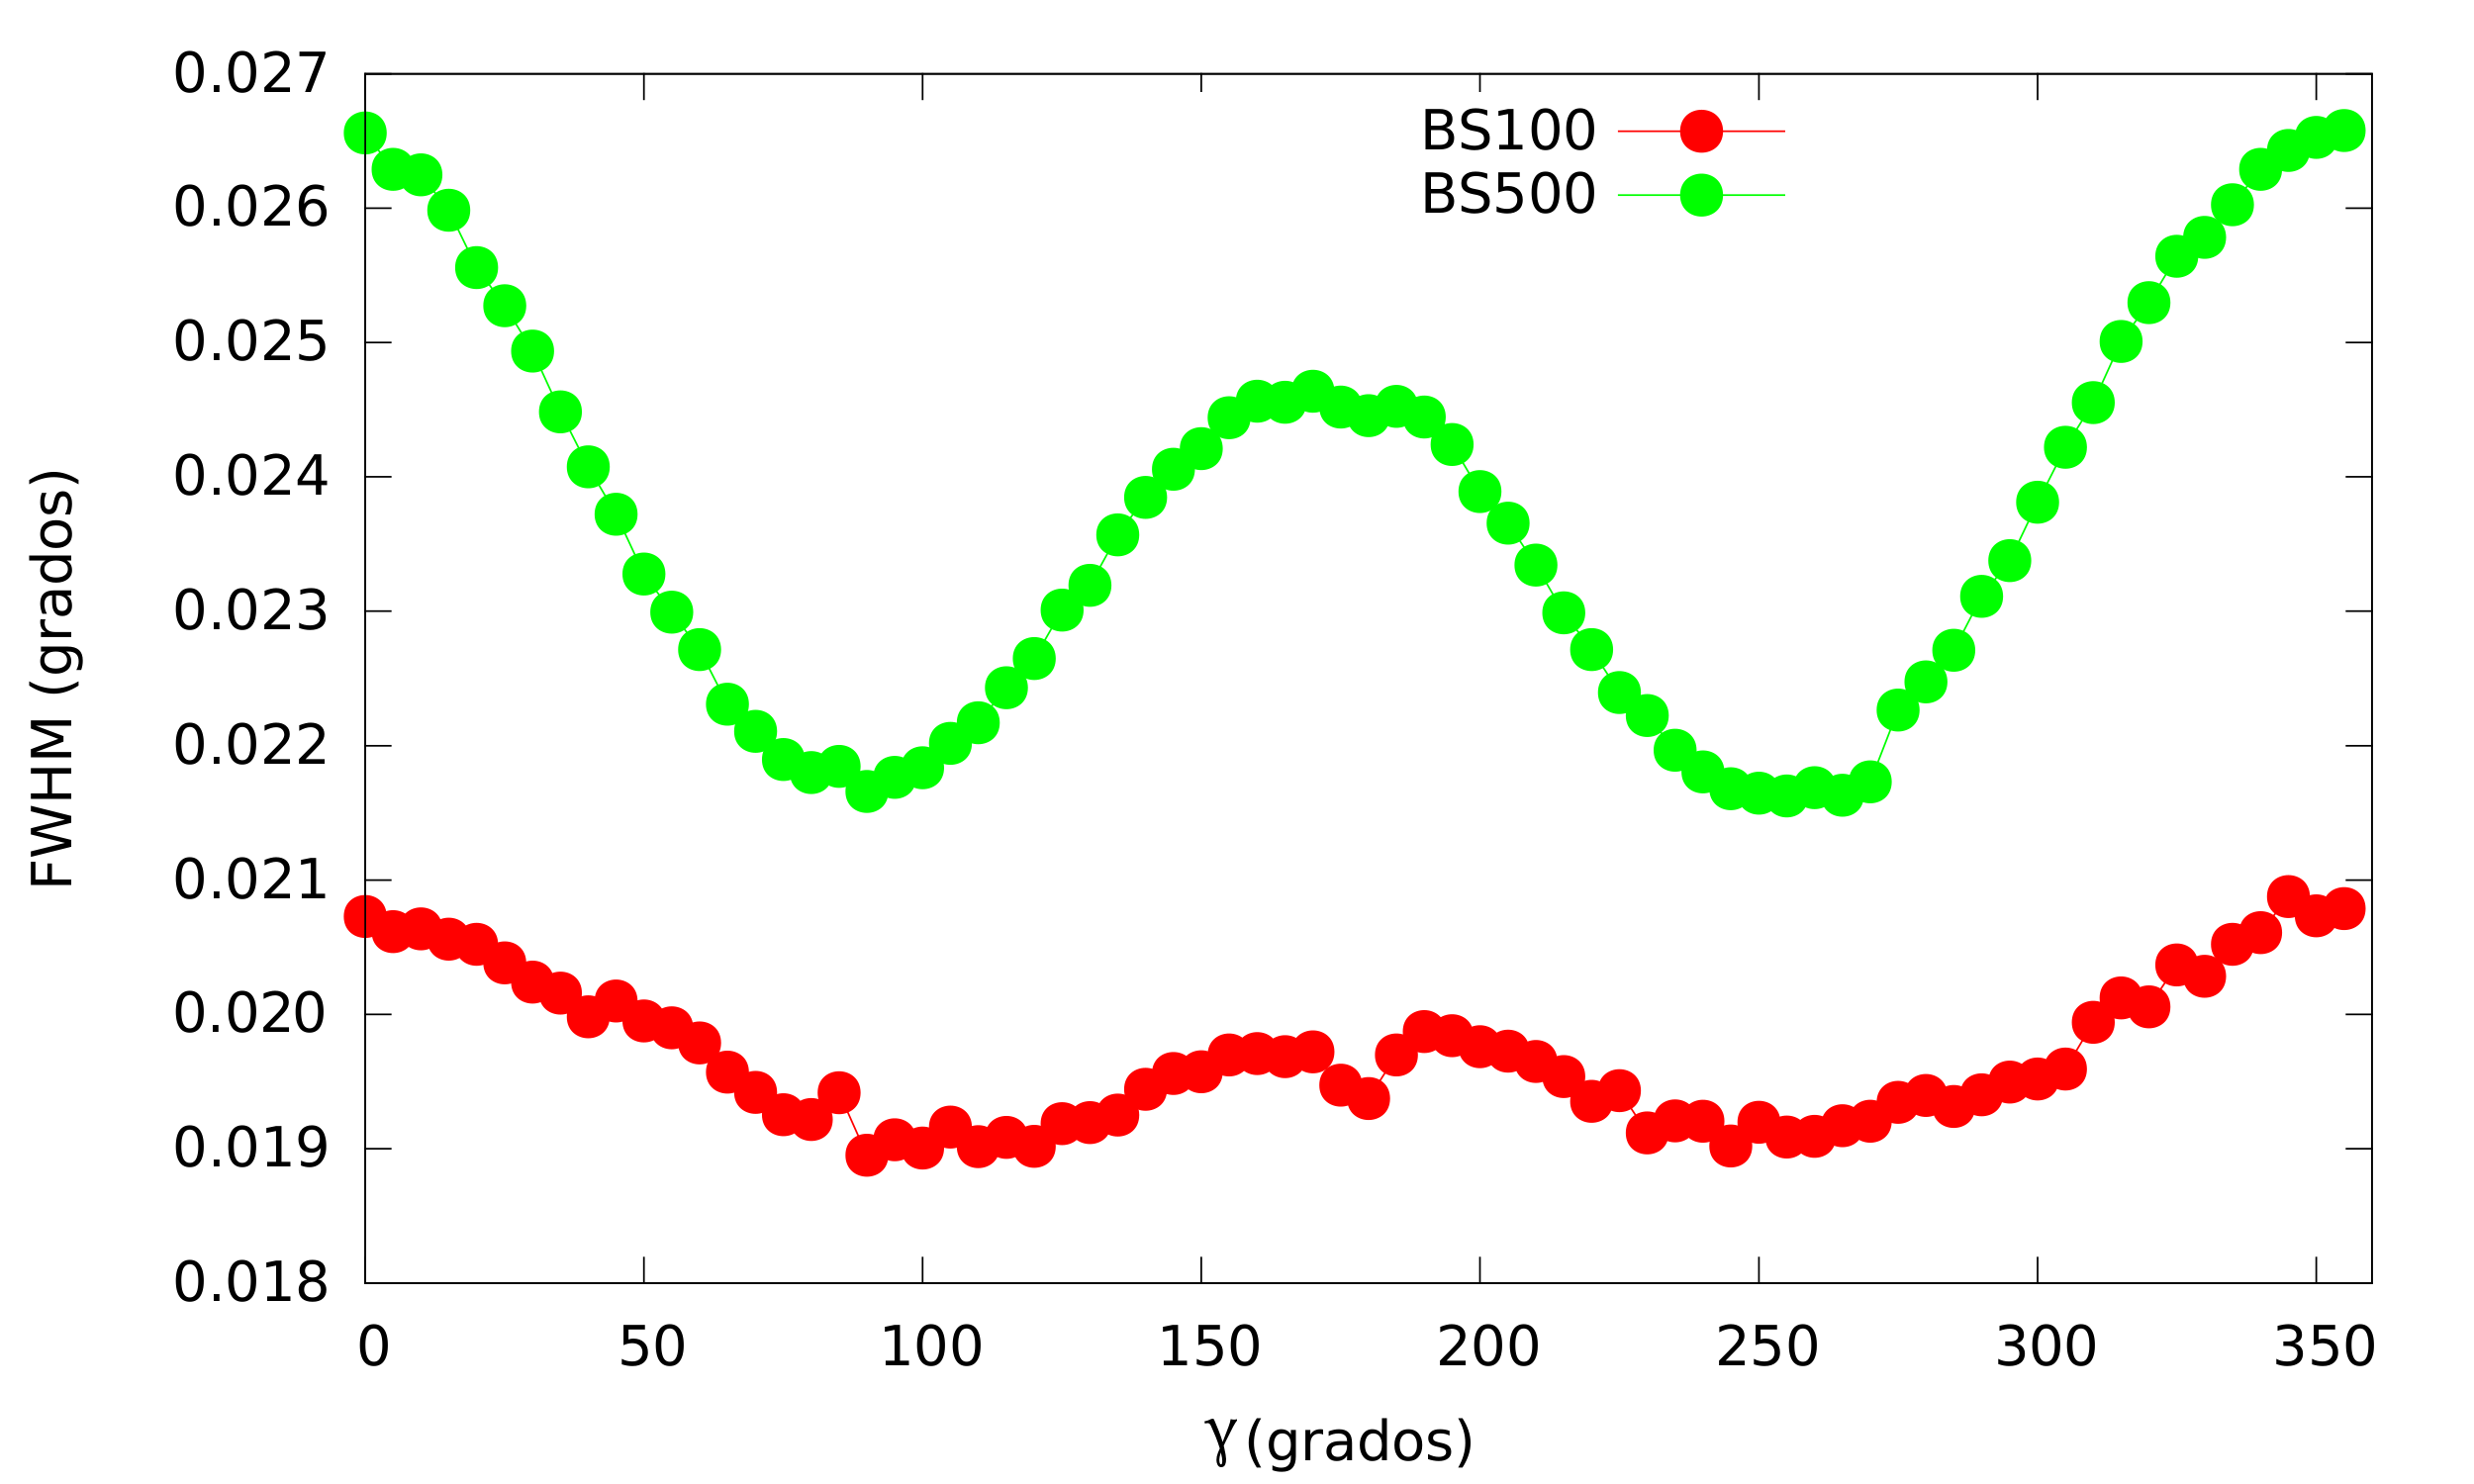
\includegraphics[width=0.8\textwidth]{LaB6_1mm_FWHMvsGammavsBS}
  \caption{Variacion del ancho instrumental como función del ángulo a lo largo del anillo de Debye.}
  \label{fig:LaB6vsGamma}
\end{figure}

\begin{figure}[!htb]
  \centering
  \includegraphics[width=0.8\textwidth]{IF75R_FWHM_Raw_Points_Sym}
  \caption{.}
  \label{fig:IF75Sym}
\end{figure}

\newpage
\subsection{Postprocesamiento de los datos}\label{SS:MatPost}
Para obtener los difractogramas necesarios tanto para medir la textura como para realizar los estudios de ancho de pico, es preciso convertir las imágenes obtenidas de los detectores de estado sólido a archivos de texto con información numérica que pueda ser procesada por programas de computadora.
Las imágenes obtenidas por el detector Mar345 fueron procesadas con el programa FIT2D\cite{FIT2D}, que permitió obtener porciones radiales con $\Delta \gamma \ = \ 5\,^{\circ}$ de ancho para cada conjunto de anillos, permitiendo obtener un difractograma para cada porción radial en la imagen registrada.
Como cada anillo barre un ángulo de 360\,$^{\circ}$, para cada ángulo $\omega$ que representa la rotación de la muestra se obtuvieron 72 difractogramas, cada uno de los cuales tenía asociada una coordenada $\gamma$, que marcaba su posición angular en la imagen extraída del programa FIT2D (Fig. \ref{fig:fit2d}).

\begin{figure}[!htb] 
  \centering
  \includegraphics[width=0.5\textwidth]{Fit2D_2}
  \caption{Para convertir las imágenes grabadas en cada experimento de difracción se empleó el programa FIT2D, que permitió dividir a cada conjunto de anillos de Debye en 72 porciones de 5\,$^{\circ}$ cada una. El programa luego extraía la intensidad de promedio grabada dentro de cada porción y con esa información construía difractogramas que fueron luego empleado para realizar los ajustes.}
  \label{fig:fit2d}
\end{figure}

Una vez obtenidos los 2664 difractogramas, los mismos fueron ajustados con un software de elaboración propia, tanto para aplicar el método de Langford como el CMWP.

Ambos softwares toman como dato de entrada todos los difractogramas obtenidos con FIT2D, además de otros archivos que deben ser escritos por el usuario, y que se encuentran ejemplificados en el apéndice \ref{CA:input}.

En el caso del programa que realiza el análisis de Langford se precisan tres archivos además de los datos extraídos de FIT2D.
El primero se denomina \textit{data\_info\_1.ini} y contiene la información que indica dónde se guardarán los resultados y dónde se encuentran los archivos de entrada, así como su cantidad y los datos necesarios para realizar la conversión angular.
También la resolución en píxeles del detector y la distancia entre el detector y la muestra, datos necesarios para convertir las distancias sobre el detector a la variable 2$\theta$.
La opción \textit{Treshold} es un dato numérico que se emplea para determinar cuál es la intensidad mínima por encima del ruido de fondo que debe tener un pico para ser ajustado por el método de mínimo cuadrados. 
Como ajustar picos de baja intensidad puede llevar a alargar el tiempo que lleva procesar los datos, además de dar resultados poco confiables, no se recomienda colocar 0 como valor de umbral, mientras que un valor de 5 ha dado buenos resultados para las mediciones realizadas en esta tesis, como se puede ver en la Fig. \ref{fig:MinIntensity}

\begin{figure}[!htb]
  \centering
  \includegraphics[width=0.8\textwidth]{Pico_minimo}
  \caption{La relación señal ruido mínima que permite distinguir y ajustar apropiadamente un pico del difractograma. El pico que se muestra tiene una intensidad integrada neta de 5 y como puede verse es ajustado razonablemente por una función pseudo-Voigt. Si el pico es más pequeño el error del ajuste se vuelve muy grande e incluso puede no converger.}
  \label{fig:MinIntensity}
\end{figure}

Las banderas \textit{Printpattern} y \textit{Correctwitdh} determinan si se van a imprimir los difractogramas extraídos junto con el mejor ajuste de cada uno, y si se van a realizar correcciones sobre el ancho de pico teniendo en cuenta el ancho de la muestra.
Esta es una característica experimental al momento de la escritura de la tesis, y debe emplearse con mucho cuidado.
Finalmente, también debe indicarse la cantidad de picos que se desean ajustar, junto con una coordenada aproximada de su centro (en 2$\theta$), los píxeles que definen inicio y final de cada pico, y dos píxeles que se determinarán el valor del ruido debajo de cada pico.

En el archivo \textit{fit\_ini\_2.ini} debe indicarse nuevamente la cantidad de picos a ajustar, así como la cantidad de puntos de ruido que se ajustarán en la rutina de mínimos cuadrados.
La rutina de mínimos cuadrados minimiza la suma total de la diferencia entre las intensidades experimentales $I_{exp}$ y las intensidades teóricas $I_{teor}$ dadas por una suma de funciones pseudo-Voigt (Ec. \ref{eq:pseudovoigt}), una por cada pico, además de un ruido que se modela como una función lineal por partes, con $N_{ruido}$ partes, cantidad que es definida por el usuario:
\begin{equation}
  I_{teor} \ = \sum_{i=1}^{N_{picos}} \ pV_i (2\theta; \ I_{0i}, 2\theta_{B_i}, H_{gl}, \eta_{gl}, sH_i, s\eta_i) \ + \sum_{j=0}^{N_{ruido}} Bg(2\theta; \ I_{B_j}, I_{B_{j+1}})
  \label{eq:Iteor}
\end{equation}
\noindent
donde la función de ruido una función lineal dentro de un intervalo definido por $2\theta_j$ y $2\theta_{j+1}$ definido por el usuario y cero fuera de ese intervalo.
La función de ruido tiene intensidad $I_j$ en el punto $2\theta_j$ e intensidad $I_{j+1}$ en el punto $2\theta_{j+1}$, y las intensidades $I_j$ e $I_{j+1}$ son ajustadas dentro de la rutina de míminos cuadrados.
De las funciones $pV(x)$, de las que hay una por pico, se ajusta su intensidad integrada $I_{0i}$, su centro $2\theta_{Bi}$ y su ancho y factor de mezcla.
El FWHM y el factor de mezcla de cada pico se generan a partir de un valor global (el mismo para todos los picos) y uno particular que se ajustan en pasos distintos del algoritmo de ajuste:

\begin{eqnarray}
  H_i & = & H_{gll} \ + \ sH_i \\
  \eta_i & = & \eta_{gl} \ + \ s\eta_i
  \label{eq:global}
\end{eqnarray}
\noindent
El motivo de esta separación es pura y exclusivamente por cuestiones de estabilidad numérica durante el ajuste, y no tiene una razón física detrás.

Todos los valores son ajustados por un rutina de mínimos cuadrados que emplea el algoritmo de Levenberg-Marquardt\cite{wiki:Levenberg} para minimizar el argumento de mínimos cuadrados:
\begin{equation}
  S(\mathbf{\chi}) \ = \ \sum_{i=1}^{N} (I^{exp}_i - I^{teor}_i(\mathbf{\chi}))^2
  \label{eq:argmin}
\end{equation}
\noindent
donde $\mathbf{\chi}$ es el conjunto de todos los parámetros que se varían para determinar la curva teórica que da el mejor ajuste a los datos experimentales.
Como el ajuste se realiza sobre cada difractograma en forma individual, $N$ indica la cantidad de mediciones que hay en un dado difractograma.

Una vez realizado el ajuste sobre todos los difractogramas, se toma la información de cada pico, el conjunto $(\theta_B, \ I_0, \ H, \ \eta)$ que tiene asociadas las coordenadas en el sistema de laboratorio $(\omega, \ \gamma, \ \theta_B)$ y se les asigna las coordenadas  $(\alpha, \ \beta)$ en el sistema de referencia del cristal, y con esos datos se construyen las figuras de polos y las figuras de polos generalizadas.
Antes de imprimir la salida de los archivos, el software substrae el ancho instrumental a partir de los valores que están presentes en el archivo \textit{IRF\_3.dat}.
Las substracción de los datos se hace suponiendo que el ancho instrumental tiene una componente Gaussiana y una componente Lorentziana, y que ambas crecen con el ánguo $\theta$ siguiendo la ley de Caglioti\cite{Caglioti1958}:
\begin{eqnarray}
  \left[H_{ins}^{G}\right]^2 & = & U_G \ \tan^2(\theta) \ + \ V_G \ \tan(\theta) \ + \ W_G \\
  H_{ins}^{L} & = & U_L \ \tan^2(\theta) \ + \ V_L \ \tan(\theta) \ + \ W_L
  \label{eq:caglioti}
\end{eqnarray}
\noindent
donde los parámetros $(U_i, V_i, W_i)$ deben ser especificados por el usuario.
En el archivo \textit{IRF\_3.dat} también deben especificarse los parámetros geométricos de la muestra para tener en cuenta la contribución del ancho de la muestra al ensanchamiento de los picos.

Los datos así obtenidos fueron procesados y graficados utilizando MTEX\cite{Hielscher2008}, un paquete de Matlab para el procesamiento de texturas.

El software que realiza el ajuste utilizando el método CMWP, tiene dos etapas básicamente: en la primera hace un ajuste al difractograma con una función como la mostrada en la Ec. \ref{eq:Iteor} y siguiendo la metodología descripta anteriormente, y usa los resultados del ajuste para generar una serie de archivos auxiliares que se necesitan para la segunda etapa.
En la segunda etapa corre en forma automática el programa CMWP siguiendo una estrategia de ajuste determinada por el usuario.

Como la primera parte de este programa funciona con un objetivo similar al del programa anterior, el primer archivo de entrada, denominado \textit{data\_info\_1.ini} es casi igual al del programa anterior, con la diferencia de que al especificar la posición de los picos a ajustar se pide que se les indique un número de fase que empieza en 0, ya que este es un dato necesario para el programa CMWP.

El segundo archivo se llama \textit{fit\_strategy\_2.ini} el usuario deber indicar los parámetros iniciales para el ajuste con pseudo-Voigts, como con el programaanterior, pero además deber indicar cuántos pasos de ajuste desea realizar con el programa CMWP, y cuáles son los coeficientes que va a ajustar en cada paso.
También debe indicar si desea que el CMWP haga un ajuste por fallas de apilamiento  y si desea que se ajuste independientemente la intensidad y posición de los picos.
En la práctica se ha visto que hacer un ajuste extra de intensidades alarga mucho el tiempo de cálculo del programa y no aporta valores finales muy diferentes a los que se obtienen cuando no se hace este ajuste.

Los siguientes tres archivos que debe generar el usuario son llamados archivos \textit{plantilla}, ya que estos archivos no suelen escribirse a mano, sino que son generados por el programa CMWP automáticamente.
En la próxima sección, donde se explica el funcionamiento del programa CMWP se explica además cómo generar los archivos plantilla.

%\begin{figure}[!htb]
%  \centering
%  \includegraphics[width=0.8\textwidth]{Conv_PF_omega_contourf}
%  \caption{Relación entre las coordenadas angulares y las coordenadas de las figuras de polos.}
%  \label{fig:LabtoPF}
%\end{figure}

\subsection{CMWP}\label{SS:CMWP}

\begin{figure}[!htb]
  \centering
  \includegraphics[width=0.8\textwidth]{CMWP_front}
  \caption{Pantalla de inicio del sofware CMWP.}
  \label{fig:CMWP_front}
\end{figure}

\newpage
\subsection{Langford}\label{SS:02Langford}

\begin{figure}[!htb]
  \centering
  \includegraphics[width=0.8\textwidth]{GaussianStrain}
  \caption{Coeficientes de strain gaussiano y lorentziano.}
  \label{fig:GaussStrainn}
\end{figure}

\begin{figure}[!htb]
  \centering
  \includegraphics[width=0.8\textwidth]{RealStrain}
  \caption{Coeficientes de strain posta.}
  \label{fig:RealStrain}
\end{figure}

\begin{figure}[!htb]
  \centering
  \includegraphics[width=0.8\textwidth]{Strain_Compare}
  \caption{Comparacion del gaussiano con el posta.}
  \label{fig:RealvsGauss}
\end{figure}

\newpage
\section{Mediciones de EBSD}\label{S:MatEBSD}
